\subsubsection{Implementation Details}

All software developed during the thesis, including the analysis and supplementary code, are developed with rigor software engineering methods.
The library components have 100\,\% unit- and integrationtest line coverage.
Each final executable is heavily tested, too.
The overall line coverage for all project code is above $98\%$.
The implementation language is C++-17\cite{c++17} and all library depdencies use at least C++-11\cite{c++11}.
All code obeys to strong typing, design by contract\cite{meyer_ieee1992} and modern idioms of the C++ programming language\cite{stroustrup_cpppl2013}.
To uncover runtime problems potentially present in C++ through raw memory access, the LLVM Address-, Memory-, Thread- and Undefined-Behaviour-Sanitizers\cite{google_sanitizers} are run over all tests.
Additional static analysis is done by clang's thread-safety analysis\cite{clang_thread_safety}, clang static analyzer\cite{clang_static_analyzer} and clang-tidy\cite{babati2017static}.
All detected issues were immediately fixed during development.
The use of continuous integration\cite{fowler_ci2000} for the whole development cycle indicated defects within hours and ensured fast development of code with a low defect rate.

The implementation goal of the developed software is to serve as a correct reference implementation for the proposed feature images.
Therefore, no special action has been taken to improve latency or throughput of the computations.
Only simple measures for speedup, namely exploiting the embarrassingly parallel nature of the processing and compiler optimizations are employed.
Figure~\ref{fig:benchmarks} shows the results of micro benchmarks of the two promising feature images.
\begin{figure}
\centering
    \begin{subfigure}[b]{0.49\linewidth}
        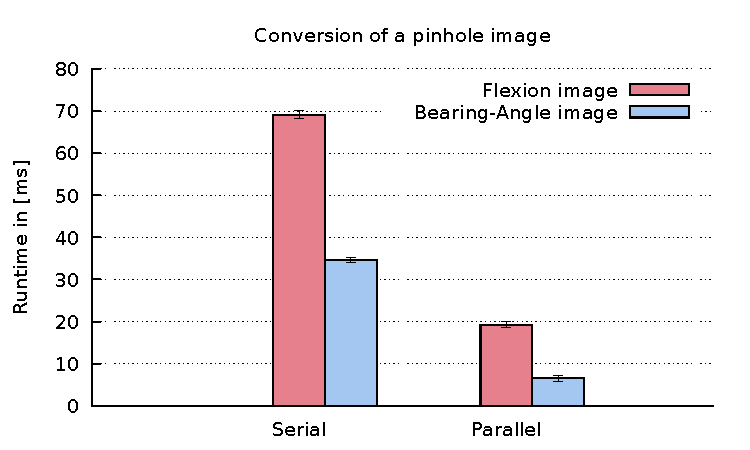
\includegraphics[width=\linewidth]{chapter06/results/benchmarks/pinhole_benchmarks.pdf}
    \end{subfigure}
    \begin{subfigure}[b]{0.49\linewidth}
        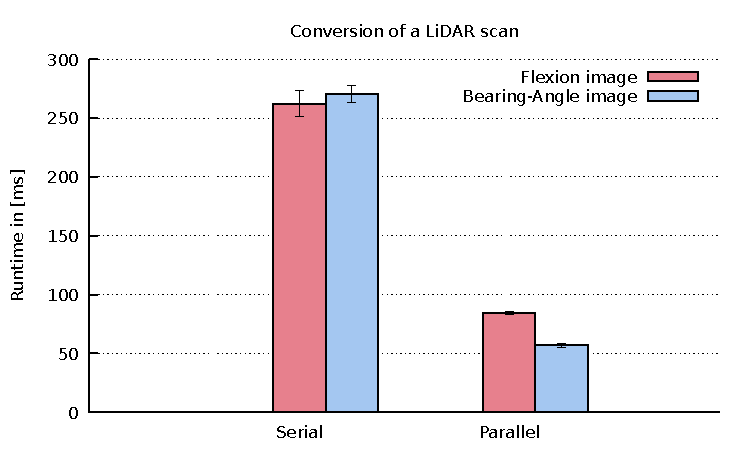
\includegraphics[width=\linewidth]{chapter06/results/benchmarks/laserscan_benchmarks.pdf}
    \end{subfigure}
    \caption[Benchmarks for Flexion and \gls{bearing-angle-image} conversions]{\emph{Benchmarks for Flexion and \gls{bearing-angle-image} conversions.} The benchmarks are run on an Intel i7-8550U with 1.8\,GHz base clock and 4 hyperthreaded cores. Each conversion is repeated 100 times for solid statistical data. The resolution of the pinhole image is 960$\times$540\,px and the \acrshort{LIDAR} scan is 3600$\times$800\,px big. The higher memory consumption of the \acrshort{LIDAR} scan results in a memory bound execution for the single threaded conversion.}\label{fig:benchmarks}
\end{figure}
Each of the feature image conversions is implemented as C++ library code working on OpenCV's\cite{opencv_library} \lstinline[basicstyle=\ttfamily]|cv::Mat| matrix type.
The conversion is generic in the sense, that any camera model implementing the forward and backward projection for pixel coordinates is suitable for the feature image conversion.
This genericity is achieved through the use of templates.
Type requirements are enforced with \lstinline[basicstyle=\ttfamily]|static_assert()| and concept-like\cite{c++concepts} requirement definitions.
One important type requirement ensures consistent use of coordinate systems with a special type that prohibits the code \texttt{\lstinline[language=C++,basicstyle=\footnotesize\ttfamily]|coordinate<float, frame::pixel> px = coordinate<float, frame::image>(0.5F, 0.25F);|} to compile.
All image access operations must adhere to the reference frame annotation and special transformations, like projections, are the only way to switch between coordinate systems.

Multiple library dependencies support the functionality of the project and shall be mentioned without a particular order.
The already mentioned OpenCV\cite{opencv_library} project provides functionality for image handling and processing. 
Required types and functionality for glue-code, parallelization and general programming utilize \emph{cli11}\cite{cli11}, \emph{rang}\cite{rang}, \emph{cpp-taskflow}\cite{Huang2019CppTaskflowFT}, \emph{fmt-lib}\cite{fmtlib}, \emph{GSL}\cite{gsl}, \emph{Eigen3}\cite{eigenweb} and \emph{Boost}\cite{boost}.
Functionality and performance testing are done with \emph{doctest}\cite{doctest} and \emph{libnonius}\cite{libnonius}.
Each used revision is documented in the code repository and differs between versions of the thesis code.
